%2multibyte Version: 5.50.0.2960 CodePage: 65001
% !TeX root = ./Slides_Lez_08_Catene_Markov.tex
% ------------------------------------------------------------
% Slides Lezione 8 - Catene di Markov: definizioni e proprieta'
% Progetto MQF - Metodi Quantitativi per la Finanza
% Macro matematiche ufficiali del progetto MQF
% Coerenti con MQF_Notazione.tex
% ------------------------------------------------------------
% Fallback utile per compilazione esterna se qualche titolo resta scritto come \QTR.
% Scientific WorkPlace usa \QTR internamente; in Beamer \QTR{frametitle}{Titolo}
% deve espandersi in \frametitle{Titolo}.

\documentclass[handout]{beamer}%
\usepackage{mathpazo}
%\usepackage{hyperref}
\usepackage{multimedia}
\usepackage{amsmath}
\usepackage{amsfonts}
\usepackage{amssymb}
\usepackage{graphicx}%
\setcounter{MaxMatrixCols}{30}
%TCIDATA{OutputFilter=latex2.dll}
%TCIDATA{Version=5.50.0.2960}
%TCIDATA{Codepage=65001}
%TCIDATA{CSTFile=beamer.cst}
%TCIDATA{<META NAME="GraphicsSave" CONTENT="32">}
%TCIDATA{<META NAME="SaveForMode" CONTENT="2">}
%TCIDATA{BibliographyScheme=Manual}
%TCIDATA{<META NAME="DocumentShell" CONTENT="Other Documents\SW\Slides - Beamer">}
%BeginMSIPreambleData
\providecommand{\U}[1]{\protect\rule{.1in}{.1in}}
%EndMSIPreambleData
\newenvironment{stepenumerate}{\begin{enumerate}[<+->]}{\end{enumerate}}
\newenvironment{stepitemize}{\begin{itemize}[<+->]}{\end{itemize} }
\newenvironment{stepenumeratewithalert}{\begin{enumerate}[<+-| alert@+>]}{\end{enumerate}}
\newenvironment{stepitemizewithalert}{\begin{itemize}[<+-| alert@+>]}{\end{itemize} }
\usetheme{Madrid}
\providecommand{\R}{\mathbb{R}}
\providecommand{\N}{\mathbb{N}}
\providecommand{\E}{\mathbb{E}}
\providecommand{\Prob}{\mathbb{P}}
\providecommand{\Q}{\mathbb{Q}}
\providecommand{\F}{\mathcal{F}}
\providecommand{\B}{\mathcal{B}}
\providecommand{\G}{\mathcal{G}}
\providecommand{\Var}{\operatorname{Var}}
\providecommand{\Cov}{\operatorname{Cov}}
\providecommand{\VaR}{\operatorname{VaR}}
\providecommand{\CVaR}{\operatorname{CVaR}}
\providecommand{\argmin}{\operatorname*{arg\,min}}
\providecommand{\argmax}{\operatorname*{arg\,max}}
\providecommand{\EVPI}{\operatorname{EVPI}}
\providecommand{\VSS}{\operatorname{VSS}}
\providecommand{\QTR}[2]{\csname #1\endcsname{#2}}
%BeginMSIPreambleData
\ifx\pdfoutput\relax\let\pdfoutput=\undefined\fi
\newcount\msipdfoutput
\ifx\pdfoutput\undefined\else
\ifcase\pdfoutput\else
\msipdfoutput=1
\ifx\paperwidth\undefined\else
\ifdim\paperheight=0pt\relax\else\pdfpageheight\paperheight\fi
\ifdim\paperwidth=0pt\relax\else\pdfpagewidth\paperwidth\fi
\fi\fi\fi
%EndMSIPreambleData


\title[Programmazione lineare]{Lezione 11 -- Programmazione lineare}
\subtitle{Metodi Quantitativi per la Finanza}
\author[P. Falbo, C. Pelizzari]{{\LARGE Paolo Falbo, Cristian Pelizzari}}
\institute[]{{\large Dipartimento di Economia e Management}}
\date[]{}
\titlegraphic{

\includegraphics[width=3.3cm]{../graphics/logo-Unibs-esteso.png}
}

\begin{document}
\maketitle

%****************************************

\section{Apertura}

\subsection{Dalla misurazione alla decisione}%

%TCIMACRO{\TeXButton{BeginFrame}{\begin{frame}}}%
%BeginExpansion
\begin{frame}%
%EndExpansion

\QTR{frametitle}{Dalla misurazione del rischio alla decisione}

%TCIMACRO{\TeXButton{Transparency}{\setbeamercovered{transparent=20}}}%
%BeginExpansion
\setbeamercovered{transparent=20}%
%EndExpansion

Nei Capitoli~8--10 le catene di Markov hanno descritto l'evoluzione degli
stati creditizi; associando a ciascuno stato una perdita monetaria, sono
state costruite distribuzioni di perdita e misure di rischio.

\medskip

{\small
\[
\begin{array}{rcl}
\mbox{Cap. 8--10} & : &
\mbox{stati futuri}\rightarrow\mbox{probabilit\`{a}}\rightarrow
\mbox{perdite}\rightarrow\mbox{misure di rischio}
\\[8pt]
\mbox{Cap. 11} & : &
\mbox{variabili decisionali}\rightarrow\mbox{vincoli}\rightarrow
\mbox{decisioni ammissibili}\\
&  &\rightarrow\mbox{scelta ottima}
\end{array}
\]
}

\medskip

\begin{stepitemize}
\item La prima catena dice quali eventi avversi possono verificarsi, con
quale probabilit\`{a} e quanto pesa la parte pi\`{u} sfavorevole della
distribuzione.

\item Non stabilisce per\`{o} \textbf{quale decisione} debba essere adottata.

\item Un intermediario deve impiegare le risorse \emph{prima} che gli eventi
futuri siano osservati: scegliere le posizioni da assumere, quante risorse
mantenere liquide, quale redditivit\`{a} perseguire.
\end{stepitemize}

%TCIMACRO{\TeXButton{Transition: Box Out}{\transboxout}}%
%BeginExpansion
\transboxout%
%EndExpansion
%TCIMACRO{\TeXButton{EndFrame}{\end{frame}}}%
%BeginExpansion
\end{frame}%
%EndExpansion

%****************************************

%TCIMACRO{\TeXButton{BeginFrame}{\begin{frame}}}%
%BeginExpansion
\begin{frame}%
%EndExpansion

\QTR{frametitle}{Percorso della lezione}

%TCIMACRO{\TeXButton{Transparency}{\setbeamercovered{transparent=20}}}%
%BeginExpansion
\setbeamercovered{transparent=20}%
%EndExpansion

\begin{stepenumerate}
\item [1.] \textbf{Formulare}: variabili decisionali, parametri, funzione
obiettivo e vincoli di un modello bancario stilizzato.

\item [2.] \textbf{Verificare}: quali composizioni dell'attivo sono
ammissibili, quali vincoli sono attivi e quali conservano un margine.

\item [3.] \textbf{Vedere}: la regione ammissibile, i punti estremi e le
rette di livello in due dimensioni.

\item [4.] \textbf{Leggere l'ottimo}: non soltanto il valore della funzione
obiettivo, ma la composizione della decisione e i vincoli che la determinano.

\item [5.] \textbf{Misurare il costo della prudenza}: di quanto si riduce il
risultato economico quando i requisiti diventano pi\`{u} severi.
\end{stepenumerate}

\medskip

\begin{center}
{\small \emph{Chiave di lettura: il vincolo non \`{e} un dettaglio tecnico
della formulazione, \`{e} la decisione.}}
\end{center}

%TCIMACRO{\TeXButton{Transition: Box Out}{\transboxout}}%
%BeginExpansion
\transboxout%
%EndExpansion
%TCIMACRO{\TeXButton{EndFrame}{\end{frame}}}%
%BeginExpansion
\end{frame}%
%EndExpansion

\section{Il caso Silicon Valley Bank}

%****************************************

\subsection{Raccolta e attivo}%

%TCIMACRO{\TeXButton{BeginFrame}{\begin{frame}}}%
%BeginExpansion
\begin{frame}%
%EndExpansion

\QTR{frametitle}{Silicon Valley Bank: la raccolta e l'attivo}

%TCIMACRO{\TeXButton{Transparency}{\setbeamercovered{transparent=20}}}%
%BeginExpansion
\setbeamercovered{transparent=20}%
%EndExpansion

\begin{stepitemize}
\item \textbf{Crescita.} Tra il 2019 e il 2021 le attivit\`{a} del gruppo
passano da circa $71$ a oltre $211$ miliardi di dollari: un volume molto
elevato di nuove risorse da investire in un periodo breve.

\item \textbf{Concentrazione della raccolta.} I depositanti appartengono in
larga parte agli stessi settori e possono manifestare esigenze di
liquidit\`{a} correlate. A fine $2022$ circa il $94\%$ dei depositi non
\`{e} coperto dall'assicurazione federale.

\item \textbf{Impieghi.} Una parte consistente delle risorse \`{e}
investita in titoli pubblici e \emph{mortgage-backed securities} a lunga
scadenza: rischio di credito contenuto, ma elevata sensibilit\`{a} alle
variazioni dei tassi.

\item \textbf{Lo scarto del $2022$.} L'aumento dei tassi riduce il valore di
mercato dei titoli lunghi; il rallentamento dei finanziamenti alle imprese
tecnologiche induce i clienti a utilizzare i depositi.
\end{stepitemize}

\medskip

\begin{center}
{\small Rischio di credito, rischio di tasso e rischio di
liquidit\`{a} sono \textbf{dimensioni distinte}: un titolo pu\`{o} essere
sicuro rispetto al rimborso del capitale e perdere valore quando i tassi
aumentano.}
\end{center}

%TCIMACRO{\TeXButton{Transition: Box Out}{\transboxout}}%
%BeginExpansion
\transboxout%
%EndExpansion
%TCIMACRO{\TeXButton{EndFrame}{\end{frame}}}%
%BeginExpansion
\end{frame}%
%EndExpansion

%***********************************************************

%****************************************

\subsection{Il meccanismo della fragilit\`{a}}%

%TCIMACRO{\TeXButton{BeginFrame}{\begin{frame}}}%
%BeginExpansion
\begin{frame}%
%EndExpansion

\QTR{frametitle}{Il meccanismo della fragilit\`{a}}

%TCIMACRO{\TeXButton{Transparency}{\setbeamercovered{transparent=20}}}%
%BeginExpansion
\setbeamercovered{transparent=20}%
%EndExpansion

\begin{center}
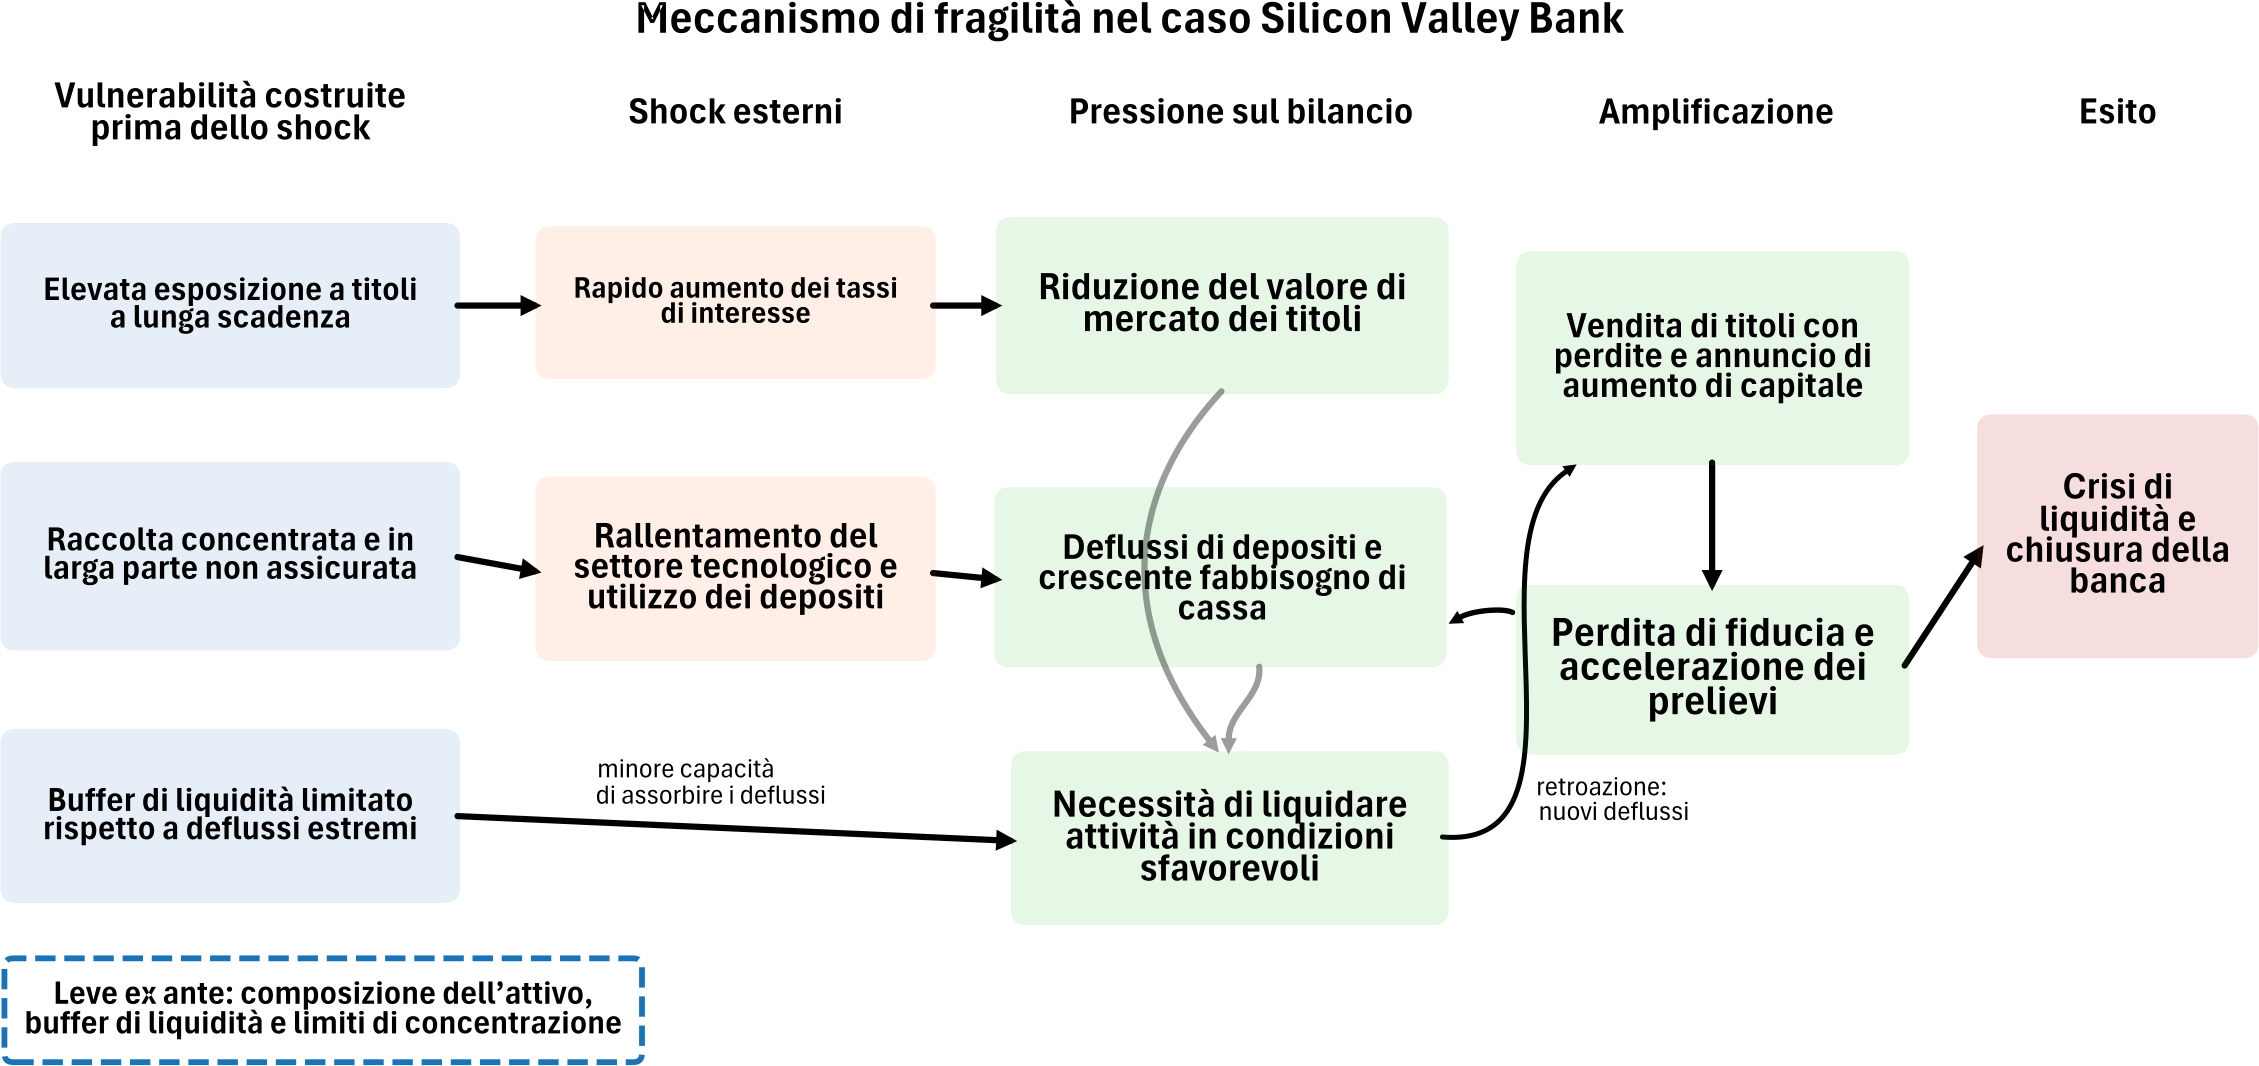
\includegraphics[width=0.90\textwidth]
{../graphics/Cap11_SVB_meccanismo_fragilita.png}
\end{center}

\medskip

\begin{stepitemize}
\item La fragilit\`{a} non dipende da una singola classe di attivo, ma
dalla \textbf{relazione} tra struttura dell'attivo e struttura della
raccolta.

\item Nel marzo $2023$ l'annuncio della vendita di una parte del
portafoglio (in perdita) rende visibili le difficolt\`{a}: il
$9$ marzo vengono richiesti prelievi per oltre $40$ miliardi, il giorno
successivo la banca viene chiusa.
\end{stepitemize}

\medskip

\begin{center}
{\small \emph{Il caso non viene usato per ricostruire il fallimento della
banca, n\'{e} si sostiene che una diversa allocazione lo avrebbe
necessariamente evitato.}}
\end{center}

%TCIMACRO{\TeXButton{Transition: Box Out}{\transboxout}}%
%BeginExpansion
\transboxout%
%EndExpansion
%TCIMACRO{\TeXButton{EndFrame}{\end{frame}}}%
%BeginExpansion
\end{frame}%
%EndExpansion

%***********************************************************

%****************************************

\subsection{Il problema guida}%

%TCIMACRO{\TeXButton{BeginFrame}{\begin{frame}}}%
%BeginExpansion
\begin{frame}%
%EndExpansion

\QTR{frametitle}{Quattro elementi, un problema decisionale}

%TCIMACRO{\TeXButton{Transparency}{\setbeamercovered{transparent=20}}}%
%BeginExpansion
\setbeamercovered{transparent=20}%
%EndExpansion

{\small
\[
\begin{array}{c}
\mbox{rapida crescita delle risorse da investire}
\\[3pt]
\mbox{concentrazione e instabilit\`{a} potenziale della raccolta}
\\[3pt]
\mbox{investimento in attivit\`{a} a lunga scadenza sensibili ai tassi}
\\[3pt]
\mbox{difficolt\`{a} di liquidazione dell'attivo in presenza di deflussi}
\end{array}
\]
}

\medskip

Considerati separatamente, questi elementi non identificano una decisione:

\begin{stepitemize}
\item pi\`{u} attivit\`{a} liquide riducono la vulnerabilit\`{a} ai
deflussi, ma tendono a ridurre la redditivit\`{a};

\item pi\`{u} titoli a lunga scadenza accrescono il rendimento corrente,
ma aumentano la sensibilit\`{a} ai tassi;

\item un limite pi\`{u} severo alle perdite migliora la resistenza allo
scenario avverso, ma restringe gli impieghi disponibili.
\end{stepitemize}

\medskip

\begin{center}
{\small \emph{Prima che una crisi si manifesti, come pu\`{o} una banca
scegliere la composizione del proprio attivo perseguendo la
redditivit\`{a}, ma rispettando simultaneamente requisiti di
liquidit\`{a}, limiti alle perdite di valore e vincoli di concentrazione?
Quale costo economico comporta rendere il bilancio pi\`{u} resiliente?}}
\end{center}

%TCIMACRO{\TeXButton{Transition: Box Out}{\transboxout}}%
%BeginExpansion
\transboxout%
%EndExpansion
%TCIMACRO{\TeXButton{EndFrame}{\end{frame}}}%
%BeginExpansion
\end{frame}%
%EndExpansion

%****************************************

\section{Variabili, parametri, risultati}

\subsection{Le variabili decisionali}%

%TCIMACRO{\TeXButton{BeginFrame}{\begin{frame}}}%
%BeginExpansion
\begin{frame}%
%EndExpansion

\QTR{frametitle}{Che cosa la banca pu\`{o} decidere}

%TCIMACRO{\TeXButton{Transparency}{\setbeamercovered{transparent=20}}}%
%BeginExpansion
\setbeamercovered{transparent=20}%
%EndExpansion

Tassi, andamento del settore tecnologico e richieste di rimborso non erano
controllabili. La \textbf{composizione dell'attivo} dipendeva invece da
decisioni gestionali. Consideriamo quattro classi aggregate:

\medskip

{\small
\[
\begin{array}{ll}
\hline
x_1 & \mbox{Cassa e riserve: disponibili subito, redditivit\`{a} minima}
\\
x_2 & \mbox{Titoli a breve: monetizzabili in tempi brevi, poco sensibili ai
tassi}
\\
x_3 & \mbox{Titoli a lunga: pi\`{u} redditizi, valore sensibile a un rialzo
dei tassi}
\\
x_4 & \mbox{Prestiti e impieghi meno liquidi: contributo elevato, non
negoziabili}
\\
\hline
\end{array}
\]
}

\medskip

\begin{stepitemize}
\item Le $x_j$ sono le \textbf{variabili decisionali}: non sono dati
osservati e non sono risultati prodotti dal modello.

\item Poich\'{e} rappresentano importi investiti, $x_j\geq0$: la
condizione esclude vendite allo scoperto e posizioni negative.

\item Una politica di allocazione \`{e} un vettore
$x=(x_1,x_2,x_3,x_4)^{\prime}$; vettori diversi sono politiche diverse.
\end{stepitemize}

%TCIMACRO{\TeXButton{Transition: Box Out}{\transboxout}}%
%BeginExpansion
\transboxout%
%EndExpansion
%TCIMACRO{\TeXButton{EndFrame}{\end{frame}}}%
%BeginExpansion
\end{frame}%
%EndExpansion


%****************************************

\subsection{I parametri}%

%TCIMACRO{\TeXButton{BeginFrame}{\begin{frame}}}%
%BeginExpansion
\begin{frame}%
%EndExpansion

\QTR{frametitle}{I dati che servono per valutare una composizione}

%TCIMACRO{\TeXButton{Transparency}{\setbeamercovered{transparent=20}}}%
%BeginExpansion
\setbeamercovered{transparent=20}%
%EndExpansion

Per ogni classe di attivo $j$ introduciamo tre coefficienti:

\medskip

{\small
\[
\begin{array}{lll}
\hline
c_j & \mbox{contributo economico unitario} &
\displaystyle\sum_{j=1}^{4}c_jx_j
\\[8pt]
q_j & \mbox{quota liquidabile entro l'orizzonte} &
\displaystyle\sum_{j=1}^{4}q_jx_j
\\[8pt]
\ell_j & \mbox{perdita unitaria nello scenario di stress} &
\displaystyle\sum_{j=1}^{4}\ell_jx_j
\\[4pt]
\hline
\end{array}
\]
}

\medskip

\begin{stepitemize}
\item $c_j$ non \`{e} necessariamente il solo tasso contrattuale: pu\`{o}
essere un margine economico atteso al netto dei costi attribuibili.

\item $q_j$ \textbf{non misura la qualit\`{a} creditizia}. Un titolo pu\`{o}
avere rischio di insolvenza minimo e non essere utile per fronteggiare
pagamenti concentrati in pochi giorni. Il coefficiente ha senso solo
rispetto a un orizzonte dichiarato.

\item I coefficienti sono \textbf{parametri}: non vengono scelti dalla
procedura di ottimizzazione, ma fissati o stimati prima della soluzione.
\end{stepitemize}

%TCIMACRO{\TeXButton{Transition: Box Out}{\transboxout}}%
%BeginExpansion
\transboxout%
%EndExpansion
%TCIMACRO{\TeXButton{EndFrame}{\end{frame}}}%
%BeginExpansion
\end{frame}%
%EndExpansion


%****************************************

\subsection{Decisioni, dati, risultati, requisiti}%

%TCIMACRO{\TeXButton{BeginFrame}{\begin{frame}}}%
%BeginExpansion
\begin{frame}%
%EndExpansion

\QTR{frametitle}{Quattro componenti da non confondere}

%TCIMACRO{\TeXButton{Transparency}{\setbeamercovered{transparent=20}}}%
%BeginExpansion
\setbeamercovered{transparent=20}%
%EndExpansion

Le tre somme della slide precedente non sono dati: sono \textbf{risultati}
della decisione. Una volta scelto $x$, possono essere calcolate.

\medskip

\begin{center}
{\small
\begin{tabular}
[c]{ll}\hline
\textbf{Variabili decisionali} & che cosa pu\`{o} essere scelto: $x_1,\ldots,x_4$\\[3pt]
\textbf{Parametri} & fissati prima della soluzione: $c_j$, $q_j$, $\ell_j$\\[3pt]
\textbf{Risultati} & che cosa discende dalla scelta: redditivit\`{a},\\
 & liquidit\`{a}, perdita sotto stress\\[3pt]
\textbf{Requisiti} & che cosa rende accettabile una decisione\\\hline
\end{tabular}
}
\end{center}

\medskip

\begin{stepitemize}
\item La banca pu\`{o} perseguire un risultato economico elevato, ma non
pu\`{o} ignorare la necessit\`{a} di mantenere liquidit\`{a} sufficiente e
di contenere le perdite potenziali.

\item Il modello dovr\`{a} quindi stabilire \emph{quale} risultato
migliorare e \emph{quali} livelli minimi o massimi rispettare.
\end{stepitemize}

\medskip

\begin{center}
{\small La programmazione lineare organizza queste quattro componenti in
un unico modello: \textbf{variabili}, \textbf{funzione obiettivo},
\textbf{vincoli}.}
\end{center}

%TCIMACRO{\TeXButton{Transition: Box Out}{\transboxout}}%
%BeginExpansion
\transboxout%
%EndExpansion
%TCIMACRO{\TeXButton{EndFrame}{\end{frame}}}%
%BeginExpansion
\end{frame}%
%EndExpansion

%*********************************

\section{Costruzione del modello}

%****************************************

\subsection{Bilancio e funzione obiettivo}%

%TCIMACRO{\TeXButton{BeginFrame}{\begin{frame}}}%
%BeginExpansion
\begin{frame}%
%EndExpansion

\QTR{frametitle}{Il vincolo di bilancio e la funzione obiettivo}

%TCIMACRO{\TeXButton{Transparency}{\setbeamercovered{transparent=20}}}%
%BeginExpansion
\setbeamercovered{transparent=20}%
%EndExpansion

Sia $A_0$ l'ammontare complessivo delle risorse da allocare. L'intero
attivo considerato deve essere distribuito tra le quattro classi:
\[
x_1+x_2+x_3+x_4=A_0.
\]

\begin{stepitemize}
\item Il vincolo non dice \emph{come} impiegare le risorse: dice soltanto
che la somma degli impieghi coincide con le risorse disponibili.

\item Le risorse non investite in titoli o prestiti sono rappresentate
dalla variabile relativa alla cassa.
\end{stepitemize}

\medskip

Se la banca intende massimizzare il risultato economico,
\[
\max\; c_1x_1+c_2x_2+c_3x_3+c_4x_4.
\]

\medskip

\begin{center}
{\small Perseguire la redditivit\`{a} \textbf{non} deve portare ad ignorare il
rischio: redditivit\`{a}, liquidit\`{a} e perdite non vengono sommate in un
unico indicatore. La prima \`{e} il risultato da migliorare, le altre
delimitano ci\`{o} che \`{e} accettabile.}
\end{center}

%TCIMACRO{\TeXButton{Transition: Box Out}{\transboxout}}%
%BeginExpansion
\transboxout%
%EndExpansion
%TCIMACRO{\TeXButton{EndFrame}{\end{frame}}}%
%BeginExpansion
\end{frame}%
%EndExpansion

%***********************************************************

%****************************************

\subsection{Il requisito di liquidit\`{a}}%

%TCIMACRO{\TeXButton{BeginFrame}{\begin{frame}}}%
%BeginExpansion
\begin{frame}%
%EndExpansion

\QTR{frametitle}{Il requisito minimo di liquidit\`{a}}

%TCIMACRO{\TeXButton{Transparency}{\setbeamercovered{transparent=20}}}%
%BeginExpansion
\setbeamercovered{transparent=20}%
%EndExpansion

La liquidit\`{a} disponibile dalla composizione $x$ entro l'orizzonte
considerato \`{e}
\[
q_1x_1+q_2x_2+q_3x_3+q_4x_4.
\]

Se $Q_{\min}$ \`{e} il livello minimo necessario per fronteggiare i
deflussi previsti nello scenario considerato,
\[
q_1x_1+q_2x_2+q_3x_3+q_4x_4\geq Q_{\min}.
\]

\medskip

\begin{stepitemize}
\item Il vincolo esclude le composizioni che, \textbf{pur essendo
redditizie}, non rendono disponibile un ammontare sufficiente di risorse
nei tempi richiesti.

\item $Q_{\min}$ non \`{e} prodotto dal modello: \`{e} una scelta
prudenziale o gestionale \textbf{prefissata}.

\item Un suo aumento restringe l'insieme delle composizioni ammissibili e
tende a spostare le risorse verso le attivit\`{a} maggiormente liquidabili.
\end{stepitemize}

\medskip

\begin{center}
{\small \`{E} il vincolo su cui torneremo: nella soluzione ottima
risulter\`{a} \textbf{attivo}, e alla fine della lezione ne misureremo il
costo.}
\end{center}

%TCIMACRO{\TeXButton{Transition: Box Out}{\transboxout}}%
%BeginExpansion
\transboxout%
%EndExpansion
%TCIMACRO{\TeXButton{EndFrame}{\end{frame}}}%
%BeginExpansion
\end{frame}%
%EndExpansion

%***********************************************************

%****************************************

\subsection{Perdite, concentrazione, non negativit\`{a}}%

%TCIMACRO{\TeXButton{BeginFrame}{\begin{frame}}}%
%BeginExpansion
\begin{frame}%
%EndExpansion

\QTR{frametitle}{Perdite sotto stress, concentrazione, non negativit\`{a}}

%TCIMACRO{\TeXButton{Transparency}{\setbeamercovered{transparent=20}}}%
%BeginExpansion
\setbeamercovered{transparent=20}%
%EndExpansion

Se $K$ \`{e} la perdita massima compatibile con la capacit\`{a}
patrimoniale,
\[
\ell_1x_1+\ell_2x_2+\ell_3x_3+\ell_4x_4\leq K.
\]

Per limitare l'esposizione verso i titoli a lunga scadenza,
\[
x_3\leq\alpha A_0,
\qquad
0\leq\alpha\leq1.
\]

\smallskip

Infine, poich\'{e} le variabili rappresentano importi investiti,
\[
x_j\geq0,
\qquad j=1,\ldots,4.
\]

\medskip

\begin{stepitemize}
\item I due limiti controllano vulnerabilit\`{a} \textbf{diverse}: il primo
l'effetto economico dello scenario di stress, il secondo la dipendenza da
una singola classe di attivo \emph{anche quando la perdita stimata resta
entro} $K$.

\item Una composizione pu\`{o} rispettare il requisito di liquidit\`{a} ed
essere comunque inammissibile perch\'{e} troppo esposta alle perdite.
\end{stepitemize}

%TCIMACRO{\TeXButton{Transition: Box Out}{\transboxout}}%
%BeginExpansion
\transboxout%
%EndExpansion
%TCIMACRO{\TeXButton{EndFrame}{\end{frame}}}%
%BeginExpansion
\end{frame}%
%EndExpansion

%***********************************************************

%****************************************

\subsection{Il modello SVB stilizzato}%

%TCIMACRO{\TeXButton{BeginFrame}{\begin{frame}}}%
%BeginExpansion
\begin{frame}%
%EndExpansion

\QTR{frametitle}{Il modello SVB stilizzato}

%TCIMACRO{\TeXButton{Transparency}{\setbeamercovered{transparent=20}}}%
%BeginExpansion
\setbeamercovered{transparent=20}%
%EndExpansion

{\small
\[
\begin{array}
[c]{ll}%
\max & c_1x_1+c_2x_2+c_3x_3+c_4x_4\\[4pt]
\text{soggetto a} & x_1+x_2+x_3+x_4=A_0,\\[3pt]
& q_1x_1+q_2x_2+q_3x_3+q_4x_4\geq Q_{\min},\\[3pt]
& \ell_1x_1+\ell_2x_2+\ell_3x_3+\ell_4x_4\leq K,\\[3pt]
& x_3\leq\alpha A_0,\\[3pt]
& x_j\geq0,\qquad j=1,\ldots,4.
\end{array}
\]
}

\medskip

\begin{center}
{\small
\begin{tabular}
[c]{lccc}\hline
\textbf{Classe di attivo} & $c_j$ & $q_j$ & $\ell_j$\\\hline
$x_1$ Cassa e riserve & $0.010$ & $1.00$ & $0.00$\\
$x_2$ Titoli a breve scadenza & $0.025$ & $0.90$ & $0.02$\\
$x_3$ Titoli a lunga scadenza & $0.040$ & $0.50$ & $0.15$\\
$x_4$ Prestiti e impieghi meno liquidi & $0.050$ & $0.20$ & $0.08$\\\hline
\end{tabular}
}
\end{center}

\smallskip

\begin{center}
{\small
$A_0=100$, \quad $Q_{\min}=55$, \quad $K=7$, \quad $\alpha=0.30$.
\smallskip

Il modello non cerca la composizione pi\`{u} redditizia in assoluto, ma la
pi\`{u} redditizia \textbf{tra quelle che rispettano simultaneamente tutti
i requisiti}.}
\end{center}

%TCIMACRO{\TeXButton{Transition: Box Out}{\transboxout}}%
%BeginExpansion
\transboxout%
%EndExpansion
%TCIMACRO{\TeXButton{EndFrame}{\end{frame}}}%
%BeginExpansion
\end{frame}%
%EndExpansion

%*****************************

\section{Linearit\`{a} e forma generale}

%****************************************

\subsection{Che cosa rende lineare il modello}%

%TCIMACRO{\TeXButton{BeginFrame}{\begin{frame}}}%
%BeginExpansion
\begin{frame}%
%EndExpansion

\QTR{frametitle}{Che cosa rende lineare il modello}

%TCIMACRO{\TeXButton{Transparency}{\setbeamercovered{transparent=20}}}%
%BeginExpansion
\setbeamercovered{transparent=20}%
%EndExpansion

Ogni variabile compare moltiplicata per un coefficiente noto e i contributi
vengono sommati. La linearit\`{a} non dipende dal fatto che il problema sia
semplice o contenga poche variabili, ma dal \textbf{modo} in cui le
decisioni entrano nella funzione obiettivo e nei vincoli.

\medskip

\begin{center}
{\small
\begin{tabular}
[c]{ll}\hline
\textbf{Proporzionalit\`{a}} & il contributo \`{e} proporzionale al
livello: $c_jx_j$, $q_jx_j$, $\ell_jx_j$\\[3pt]
\textbf{Additivit\`{a}} & il risultato \`{e} la somma dei contributi, senza
interazioni\\[3pt]
\textbf{Divisibilit\`{a}} & le variabili assumono valori reali non
negativi\\[3pt]
\textbf{Coefficienti} & $c_j$, $q_j$, $\ell_j$ e i livelli $A_0$,
$Q_{\min}$, $K$, $\alpha$\\
\quad \textbf{come parametri} & sono fissati prima della soluzione\\\hline
\end{tabular}
}
\end{center}

\medskip

\begin{stepitemize}
\item Nel caso SVB: rendimento, quota liquidabile e perdita unitaria
attribuiti a una classe \textbf{non cambiano} al variare dell'importo
investito.

\item La divisibilit\`{a} \`{e} naturale per importi monetari; non lo
sarebbe per decisioni indivisibili, che richiederebbero variabili intere.
\end{stepitemize}

%TCIMACRO{\TeXButton{Transition: Box Out}{\transboxout}}%
%BeginExpansion
\transboxout%
%EndExpansion
%TCIMACRO{\TeXButton{EndFrame}{\end{frame}}}%
%BeginExpansion
\end{frame}%
%EndExpansion

%***********************************************************

%****************************************

\subsection{Che cosa la linearit\`{a} esclude}%

%TCIMACRO{\TeXButton{BeginFrame}{\begin{frame}}}%
%BeginExpansion
\begin{frame}%
%EndExpansion

\QTR{frametitle}{Che cosa la linearit\`{a} esclude}

%TCIMACRO{\TeXButton{Transparency}{\setbeamercovered{transparent=20}}}%
%BeginExpansion
\setbeamercovered{transparent=20}%
%EndExpansion

Non compaiono potenze delle variabili, prodotti tra variabili, coefficienti
dipendenti dalle quantit\`{a} investite. Non sarebbero lineari
\[
x_3^2,
\qquad
x_2x_3,
\qquad
c_3(x_3)\,x_3.
\]

\medskip

\begin{stepitemize}
\item \textbf{Nessuna amplificazione.} Il modello non considera che
un'esposizione simultanea verso titoli a lunga e prestiti poco liquidi
possa produrre una vulnerabilit\`{a} superiore alla somma delle due: un
termine $\gamma x_3x_4$ renderebbe il modello non lineare.

\item \textbf{No fire sale.} La vendita di una grande posizione
pu\`{o} deprimere il prezzo: la perdita unitaria non resta costante al
crescere dell'importo liquidato. Servirebbe $L_j=L_j(x_j)$.

\item \textbf{L'incertezza non scompare}, viene incorporata nei
coefficienti. Il modello risponde a una domanda condizionata: qual \`{e} la
migliore allocazione \emph{se} i coefficienti e lo scenario di stress
assumono i valori indicati.
\end{stepitemize}

\medskip

%TCIMACRO{\TeXButton{Transition: Box Out}{\transboxout}}%
%BeginExpansion
\transboxout%
%EndExpansion
%TCIMACRO{\TeXButton{EndFrame}{\end{frame}}}%
%BeginExpansion
\end{frame}%
%EndExpansion

%****************************************

%****************************************

\subsection{Dalla forma scalare alla forma matriciale}%

%TCIMACRO{\TeXButton{BeginFrame}{\begin{frame}}}%
%BeginExpansion
\begin{frame}%
%EndExpansion

\QTR{frametitle}{Dal caso SVB alla formulazione generale}

%TCIMACRO{\TeXButton{Transparency}{\setbeamercovered{transparent=20}}}%
%BeginExpansion
\setbeamercovered{transparent=20}%
%EndExpansion

La struttura non dipende dal numero di classi. Con $n$ variabili e $m$
requisiti:
\[
\begin{array}
[c]{ll}%
\max & \displaystyle\sum_{j=1}^{n}c_jx_j\\[10pt]
\text{soggetto a} & \displaystyle\sum_{j=1}^{n}a_{ij}x_j\leq b_i,
\qquad i=1,\ldots,m,\\[8pt]
& x_j\geq0,\qquad j=1,\ldots,n.
\end{array}
\]

Raccogliendo $x$, $c$, $b$ e la matrice $A=(a_{ij})$:
\[
\begin{array}
[c]{ll}%
\max\limits_x & c^{\prime}x\\[4pt]
\text{soggetto a} & Ax\leq b,\\[2pt]
& x\geq0.
\end{array}
\]

\medskip

\begin{stepitemize}
\item Ogni \textbf{riga} di $A$ \`{e} un requisito; ogni \textbf{colonna}
descrive come una variabile contribuisce ai diversi requisiti. Nel modello
SVB una colonna riassume redditivit\`{a}, liquidabilit\`{a} e perdita sotto
stress di una classe di attivo.

\end{stepitemize}

%TCIMACRO{\TeXButton{Transition: Box Out}{\transboxout}}%
%BeginExpansion
\transboxout%
%EndExpansion
%TCIMACRO{\TeXButton{EndFrame}{\end{frame}}}%
%BeginExpansion
\end{frame}%
%EndExpansion

%*****************************
\section{Decisioni ammissibili e diagnosi}

%*****************************

\subsection{Decisioni ammissibili}%

%TCIMACRO{\TeXButton{BeginFrame}{\begin{frame}}}%
%BeginExpansion
\begin{frame}%
%EndExpansion

\QTR{frametitle}{Quali composizioni possono essere considerate}

%TCIMACRO{\TeXButton{Transparency}{\setbeamercovered{transparent=20}}}%
%BeginExpansion
\setbeamercovered{transparent=20}%
%EndExpansion

Una composizione $\bar{x}$ \`{e} \textbf{ammissibile} se soddisfa
\emph{tutti} i vincoli del modello: bilancio, requisito di liquidit\`{a},
limite alle perdite, limite di concentrazione e non negativit\`{a}.

\medskip

L'insieme delle soluzioni ammissibili si indica con $\mathcal{X}$; nella
formulazione generale
\[
\mathcal{X}=\left\{ x\in\R^n:Ax\leq b,\;x\geq0\right\} .
\]

La funzione obiettivo viene massimizzata \textbf{non} su tutto $\R^n$, ma
su $\mathcal{X}$:
\[
z^{*}=\max_{x\in\mathcal{X}}c^{\prime}x.
\]

\medskip

\begin{stepitemize}
\item Il rispetto di un \emph{singolo} requisito non rende ammissibile una
decisione: una composizione pu\`{o} avere liquidit\`{a} sufficiente e
produrre nello stesso tempo una perdita eccessiva sotto stress.

\item Una decisione con risultato economico molto elevato ma esterna a
$\mathcal{X}$ non \`{e} un'alternativa migliore: \`{e} una decisione che il
modello considera \textbf{non realizzabile}.
\end{stepitemize}

%TCIMACRO{\TeXButton{Transition: Box Out}{\transboxout}}%
%BeginExpansion
\transboxout%
%EndExpansion
%TCIMACRO{\TeXButton{EndFrame}{\end{frame}}}%
%BeginExpansion
\end{frame}%
%EndExpansion

%*****************************

\subsection{Margine e vincoli attivi}%

%TCIMACRO{\TeXButton{BeginFrame}{\begin{frame}}}%
%BeginExpansion
\begin{frame}%
%EndExpansion

\QTR{frametitle}{Due composizioni a confronto}

%TCIMACRO{\TeXButton{Transparency}{\setbeamercovered{transparent=20}}}%
%BeginExpansion
\setbeamercovered{transparent=20}%
%EndExpansion

Con $A_0=100$, $Q_{\min}=55$, $K=7$, $\alpha A_0=30$:

\medskip

\begin{center}
{\small
\begin{tabular}
[c]{lcccc}\hline
& \textbf{Risultato} & \textbf{Liquidit\`{a}} & \textbf{Perdita} &
\textbf{Titoli lunghi}\\\hline
$x^{(A)}=(5,10,45,40)^{\prime}$ & $4.10$ & $44.50$ & $10.15$ & $45$\\
$x^{(B)}=(10,30,20,40)^{\prime}$ & $3.65$ & $55.00$ & $6.80$ & $20$\\\hline
\multicolumn{1}{r}{\emph{richiesto}} & & $\geq55$ & $\leq7$ & $\leq30$\\
\end{tabular}
}
\end{center}

\medskip

\begin{stepitemize}
\item $x^{(A)}$ produce il risultato pi\`{u} elevato e viola
\textbf{tre} requisiti. Non pu\`{o} essere preferita a $x^{(B)}$: la
verifica dell'ammissibilit\`{a} \textbf{precede} il confronto dei valori
della funzione obiettivo.

\item Per $x^{(B)}$ i margini sono $55-55=0$ sulla liquidit\`{a},
$7-6.80=0.20$ sulla perdita, $30-20=10$ sulla concentrazione.
\end{stepitemize}

\medskip

Un vincolo \`{e} \textbf{attivo} quando \`{e} soddisfatto esattamente al
proprio limite, cio\`{e} quando il suo margine \`{e} nullo. In $x^{(B)}$ il
requisito di liquidit\`{a} \`{e} attivo: ridurre le attivit\`{a} liquide,
a parit\`{a} del resto, renderebbe la decisione inammissibile.

%TCIMACRO{\TeXButton{Transition: Box Out}{\transboxout}}%
%BeginExpansion
\transboxout%
%EndExpansion
%TCIMACRO{\TeXButton{EndFrame}{\end{frame}}}%
%BeginExpansion
\end{frame}%
%EndExpansion

%*****************************

\subsection{I tre esiti del solver}%

%TCIMACRO{\TeXButton{BeginFrame}{\begin{frame}}}%
%BeginExpansion
\begin{frame}%
%EndExpansion

\QTR{frametitle}{Che cosa pu\`{o} rispondere un solver}

%TCIMACRO{\TeXButton{Transparency}{\setbeamercovered{transparent=20}}}%
%BeginExpansion
\setbeamercovered{transparent=20}%
%EndExpansion

\begin{stepenumerate}
\item [1.] Una \textbf{soluzione ottima} e il corrispondente valore
obiettivo.

\item [2.] L'\textbf{inammissibilit\`{a}} del modello, cio\`{e}
$\mathcal{X}=\varnothing$: nessuna decisione soddisfa simultaneamente tutti
i vincoli.

\item [3.] L'\textbf{illimitatezza}: esistono decisioni ammissibili che
producono valori arbitrariamente elevati. In un problema finanziario
segnala normalmente che manca un vincolo rilevante.
\end{stepenumerate}

\medskip

Nel problema bancario una regione vuota pu\`{o} indicare requisiti
incompatibili con le attivit\`{a} disponibili, un limite alle perdite
troppo restrittivo, limiti di concentrazione che impediscono di impiegare
l'attivo, \emph{oppure} dati e vincoli formulati in modo incoerente.

\medskip

\begin{center}
{\small \emph{La prima operazione da compiere quando un solver dichiara il
problema inammissibile non \`{e} modificare i vincoli fino a ottenere una
soluzione. Occorre identificare quali requisiti sono incompatibili e
stabilire se l'incompatibilit\`{a} derivi dal problema economico o dalla
sua formulazione.}}
\end{center}

%TCIMACRO{\TeXButton{Transition: Box Out}{\transboxout}}%
%BeginExpansion
\transboxout%
%EndExpansion
%TCIMACRO{\TeXButton{EndFrame}{\end{frame}}}%
%BeginExpansion
\end{frame}%
%EndExpansion

%*****************************

\section{Esercizio in aula: verifica di ammissibilit\`{a}}

%*****************************

\subsection{Enunciato}%

%TCIMACRO{\TeXButton{BeginFrame}{\begin{frame}}}%
%BeginExpansion
\begin{frame}%
%EndExpansion

\QTR{frametitle}{Esercizio: questa composizione \`{e} ammissibile?}

%TCIMACRO{\TeXButton{Transparency}{\setbeamercovered{transparent=20}}}%
%BeginExpansion
\setbeamercovered{transparent=20}%
%EndExpansion

Modello bancario con $A_0=100$, $Q_{\min}=55$, $K=7$, $\alpha A_0=30$. Si
consideri la composizione
\[
x=(8,\;32,\;18,\;42)^{\prime}.
\]

\medskip

\begin{stepenumerate}
\item [1.] Verificare il vincolo di bilancio.

\item [2.] Calcolare la liquidit\`{a} disponibile e la perdita nello
scenario di stress.

\item [3.] Stabilire se la composizione \`{e} ammissibile e, in caso
negativo, quale requisito \`{e} violato.

\item [4.] Per ciascun requisito rispettato, calcolare il margine e dire se
il vincolo \`{e} attivo.
\end{stepenumerate}

\medskip

\begin{center}
{\small
$q=(1.00,\;0.90,\;0.50,\;0.20)$
\qquad
$\ell=(0,\;0.02,\;0.15,\;0.08)$}
\end{center}

%TCIMACRO{\TeXButton{Transition: Box Out}{\transboxout}}%
%BeginExpansion
\transboxout%
%EndExpansion
%TCIMACRO{\TeXButton{EndFrame}{\end{frame}}}%
%BeginExpansion
\end{frame}%
%EndExpansion

%*****************************

\subsection{Il calcolo}%

%TCIMACRO{\TeXButton{BeginFrame}{\begin{frame}}}%
%BeginExpansion
\begin{frame}%
%EndExpansion

\QTR{frametitle}{Le tre grandezze prodotte dalla composizione}

%TCIMACRO{\TeXButton{Transparency}{\setbeamercovered{transparent=20}}}%
%BeginExpansion
\setbeamercovered{transparent=20}%
%EndExpansion

Bilancio:
\[
8+32+18+42=100=A_0.
\]

Liquidit\`{a} disponibile:
\[
1.00(8)+0.90(32)+0.50(18)+0.20(42)=8+28.8+9+8.4=54.2.
\]

Perdita nello scenario di stress:
\[
0.02(32)+0.15(18)+0.08(42)=0.64+2.70+3.36=6.70.
\]

\medskip

\begin{stepitemize}
\item Il bilancio \`{e} un'uguaglianza: \`{e} soddisfatto esattamente da
ogni composizione che impieghi tutte le risorse.

\item La cassa non contribuisce alla perdita, perch\'{e} $\ell_1=0$:
compare nella liquidit\`{a} con coefficiente unitario e nella perdita non
compare affatto.
\end{stepitemize}

%TCIMACRO{\TeXButton{Transition: Box Out}{\transboxout}}%
%BeginExpansion
\transboxout%
%EndExpansion
%TCIMACRO{\TeXButton{EndFrame}{\end{frame}}}%
%BeginExpansion
\end{frame}%
%EndExpansion

%*****************************

\subsection{La diagnosi}%

%TCIMACRO{\TeXButton{BeginFrame}{\begin{frame}}}%
%BeginExpansion
\begin{frame}%
%EndExpansion

\QTR{frametitle}{Valore, limite, margine}

%TCIMACRO{\TeXButton{Transparency}{\setbeamercovered{transparent=20}}}%
%BeginExpansion
\setbeamercovered{transparent=20}%
%EndExpansion

\begin{center}
{\small
\begin{tabular}
[c]{lccc}\hline
\textbf{Requisito} & \textbf{Valore} & \textbf{Limite} & \textbf{Margine}%
\\\hline
Liquidit\`{a} & $54.2$ & $\geq55$ & $-0.8$ \quad violato\\
Perdita sotto stress & $6.70$ & $\leq7$ & $0.30$\\
Titoli a lunga scadenza & $18$ & $\leq30$ & $12$\\\hline
\end{tabular}
}
\end{center}

\medskip

\begin{stepitemize}
\item Un solo requisito violato basta: $x\notin\mathcal{X}$. Il risultato
economico della composizione non viene nemmeno calcolato.

\item Nessun vincolo \`{e} attivo tra quelli rispettati: entrambi
conservano margine. La composizione non si trova su alcuna frontiera.

\item Lo scostamento $-0.8$ misura quanta liquidit\`{a} manca. \`{E} la
quantit\`{a} che una correzione dovrebbe colmare.
\end{stepitemize}

%TCIMACRO{\TeXButton{Transition: Box Out}{\transboxout}}%
%BeginExpansion
\transboxout%
%EndExpansion
%TCIMACRO{\TeXButton{EndFrame}{\end{frame}}}%
%BeginExpansion
\end{frame}%
%EndExpansion

%*****************************

\section{La geometria del problema}

%*****************************

\subsection{Un modello bancario ridotto}%

%TCIMACRO{\TeXButton{BeginFrame}{\begin{frame}}}%
%BeginExpansion
\begin{frame}%
%EndExpansion

\QTR{frametitle}{Un problema bancario ridotto, rappresentabile graficamente}

%TCIMACRO{\TeXButton{Transparency}{\setbeamercovered{transparent=20}}}%
%BeginExpansion
\setbeamercovered{transparent=20}%
%EndExpansion

Il modello a quattro classi non pu\`{o} essere rappresentato su un piano.
Consideriamo una versione ridotta a \textbf{due sole grandezze}: le
attivit\`{a} liquide e i titoli a lunga scadenza.

\medskip

\begin{center}
{\small
\begin{tabular}
[c]{ll}\hline
$x_1$ & attivit\`{a} liquide\\
$x_2$ & titoli a lunga scadenza\\\hline
\end{tabular}
}
\end{center}

\begin{center}
{\small \emph{Avvertenza: in questa rappresentazione le due variabili sono
ridefinite. }}
\end{center}

\medskip

\begin{stepitemize}
\item Le risorse destinate alle due classi non possono superare $A_0$: la
parte restante \`{e} investita nelle altre classi, non rappresentate.

\item Restano un requisito minimo sulle liquide e un limite massimo sulle
lunghe, oltre alla non negativit\`{a}.
\end{stepitemize}
\[
x_1+x_2\leq10,
\qquad
x_1\geq3,
\qquad
x_2\leq4,
\qquad
x_1,x_2\geq0.
\]


%TCIMACRO{\TeXButton{Transition: Box Out}{\transboxout}}%
%BeginExpansion
\transboxout%
%EndExpansion
%TCIMACRO{\TeXButton{EndFrame}{\end{frame}}}%
%BeginExpansion
\end{frame}%
%EndExpansion

%*****************************

\subsection{Regione ammissibile e vertici}%

%TCIMACRO{\TeXButton{BeginFrame}{\begin{frame}}}%
%BeginExpansion
\begin{frame}%
%EndExpansion

\QTR{frametitle}{La regione ammissibile e i suoi vertici}

%TCIMACRO{\TeXButton{Transparency}{\setbeamercovered{transparent=20}}}%
%BeginExpansion
\setbeamercovered{transparent=20}%
%EndExpansion

\begin{center}
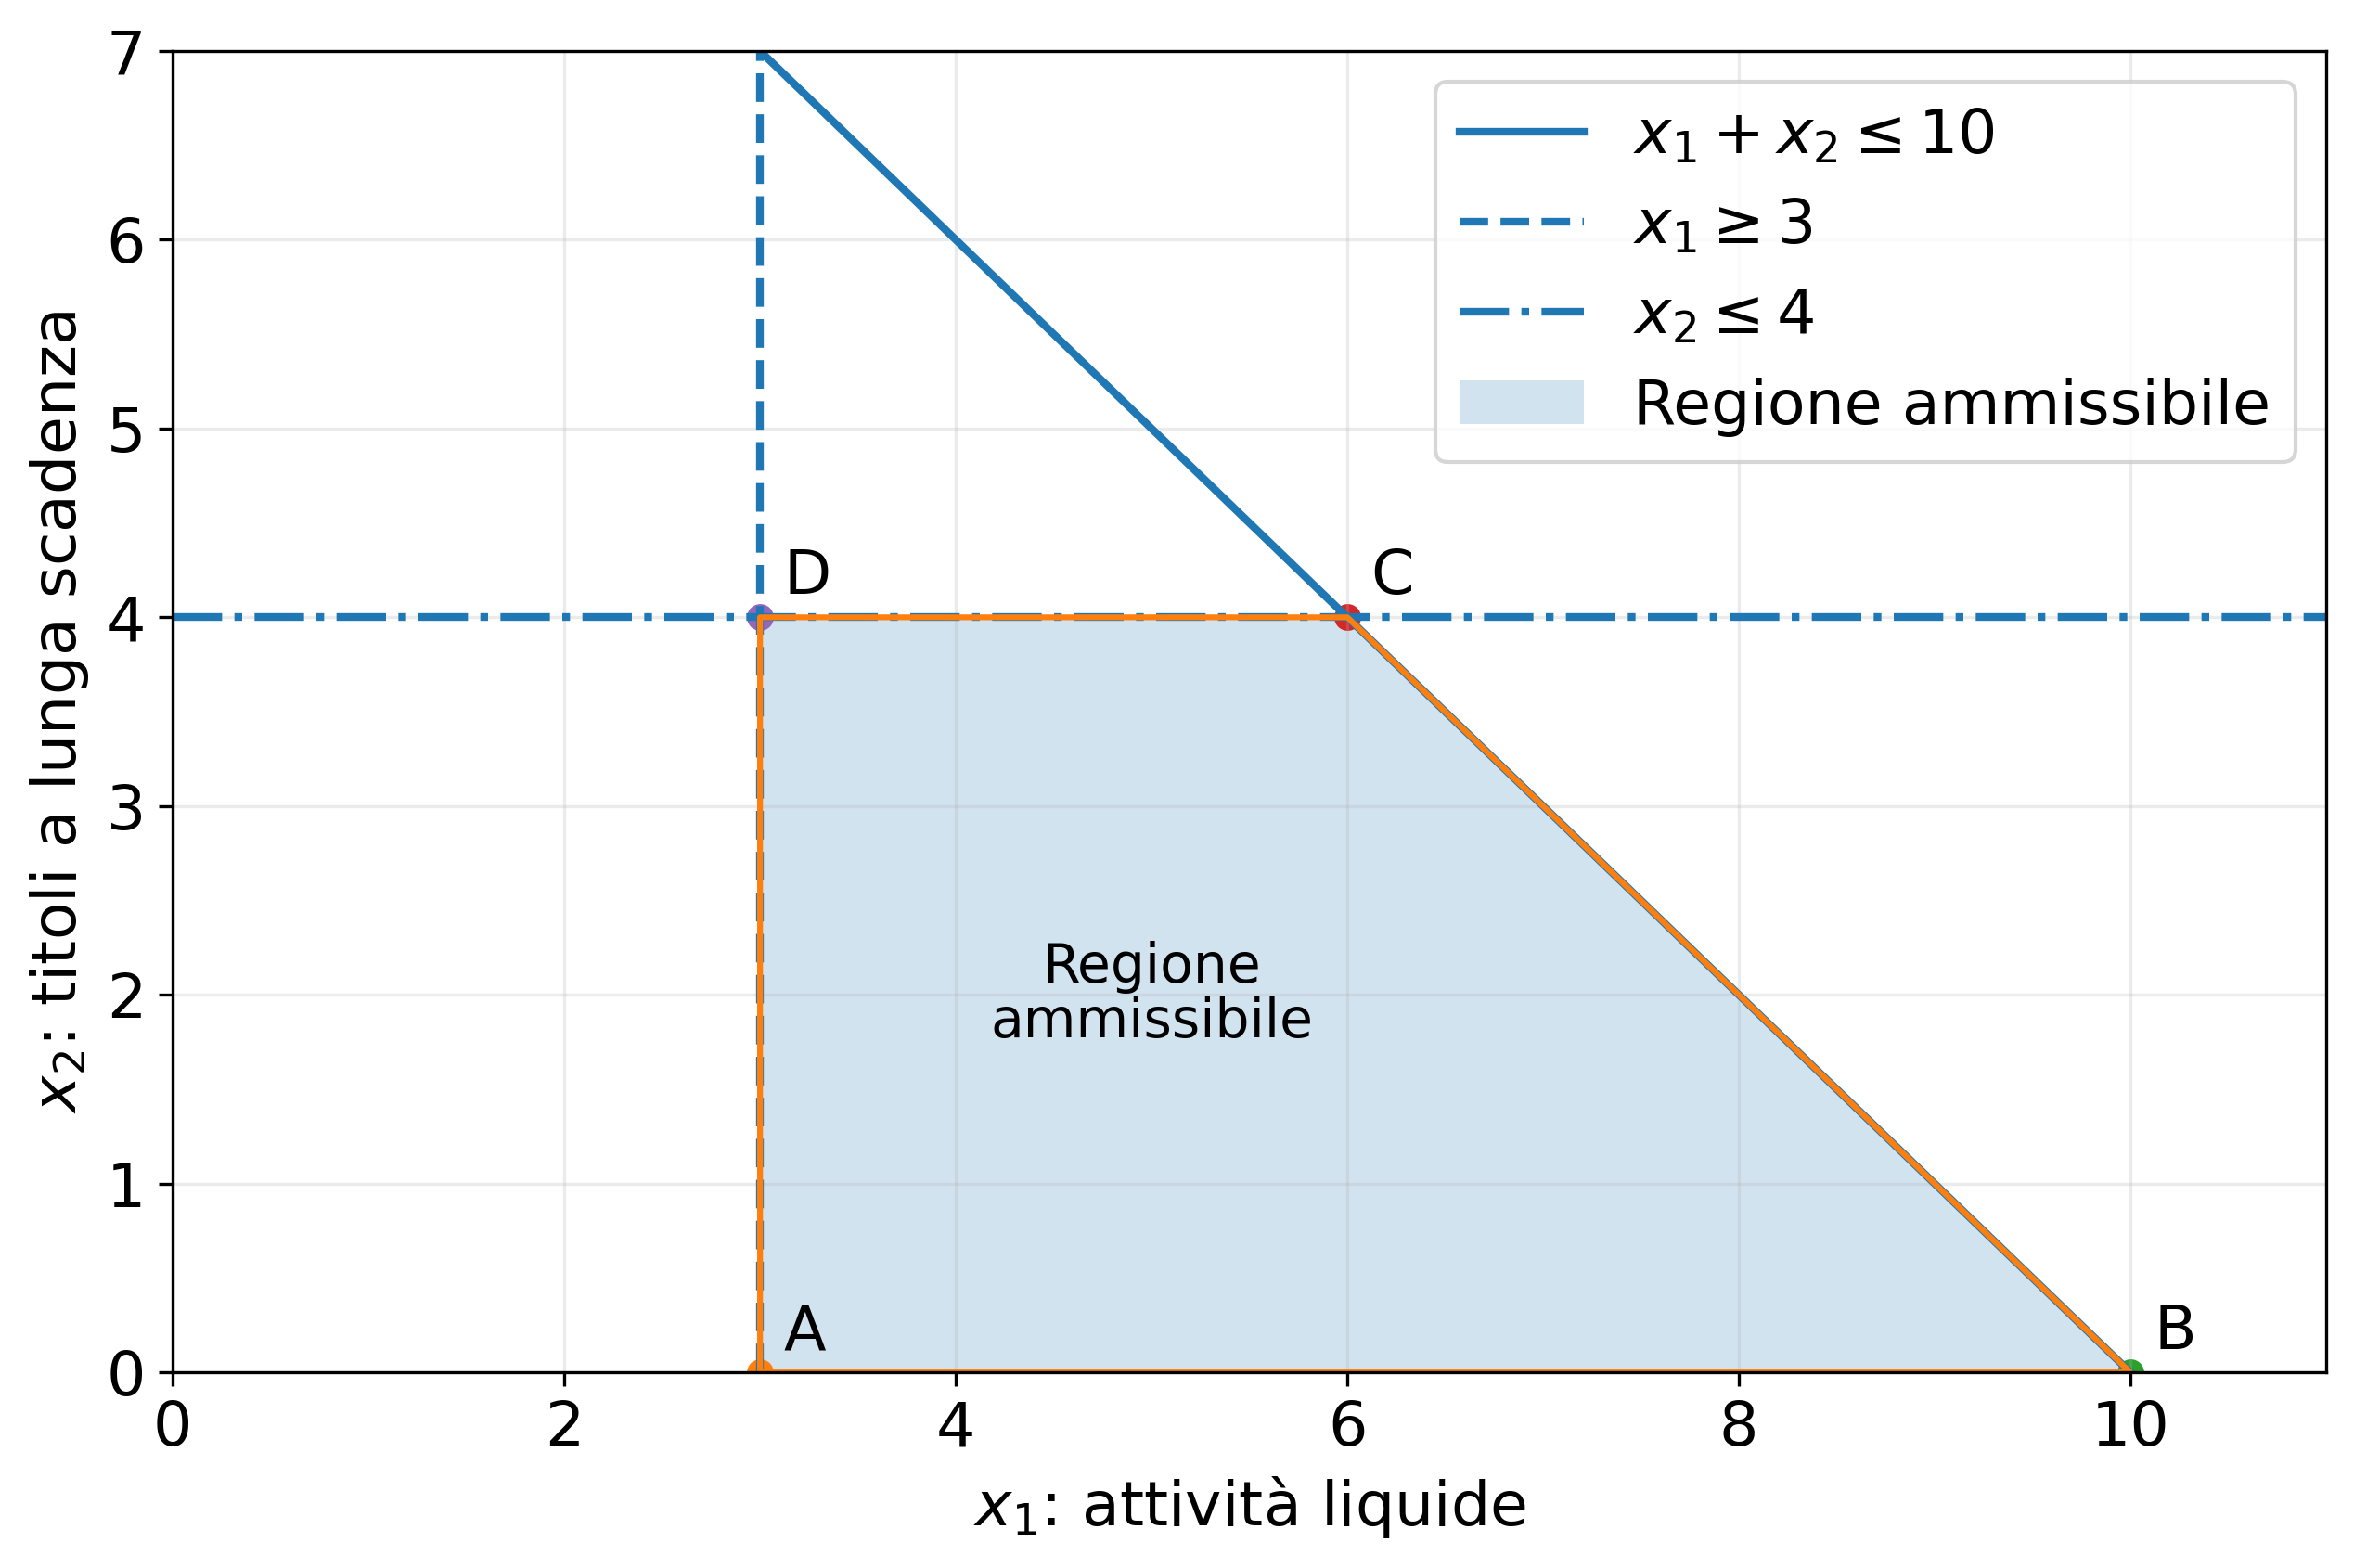
\includegraphics[width=0.62\textwidth]
{../graphics/cap11_geometria_programmazione_lineare.png}
\end{center}

\begin{center}
{\small
\begin{tabular}
[c]{ccl}\hline
\textbf{Vertice} & \textbf{Coordinate} & \textbf{Vincoli attivi}\\\hline
$A$ & $(3,0)$ & liquide al minimo, nessuna lunga\\
$B$ & $(10,0)$ & risorse esaurite, nessuna lunga\\
$C$ & $(6,4)$ & risorse esaurite, lunghe al massimo\\
$D$ & $(3,4)$ & liquide al minimo, lunghe al massimo\\\hline
\end{tabular}
}
\end{center}

%TCIMACRO{\TeXButton{Transition: Box Out}{\transboxout}}%
%BeginExpansion
\transboxout%
%EndExpansion
%TCIMACRO{\TeXButton{EndFrame}{\end{frame}}}%
%BeginExpansion
\end{frame}%
%EndExpansion

%*****************************

\subsection{Rette di livello e punti estremi}%

%TCIMACRO{\TeXButton{BeginFrame}{\begin{frame}}}%
%BeginExpansion
\begin{frame}%
%EndExpansion

\QTR{frametitle}{Come la funzione obiettivo sceglie un vertice}

%TCIMACRO{\TeXButton{Transparency}{\setbeamercovered{transparent=20}}}%
%BeginExpansion
\setbeamercovered{transparent=20}%
%EndExpansion

Fissato un livello $k$, l'equazione $c_1x_1+c_2x_2=k$ descrive una
\textbf{retta di livello}: tutti i suoi punti danno lo stesso risultato. Al
crescere di $k$ la retta trasla parallelamente; la soluzione ottima \`{e}
l'ultimo punto di contatto con la regione.

\medskip

Confrontando i due vertici pi\`{u} lontani nella direzione di crescita:
\[
z(B)=10c_1,
\qquad
z(C)=6c_1+4c_2.
\]

\begin{stepitemize}
\item Se le lunghe rendono pi\`{u} delle liquide, vince $C$; nel caso
opposto vince $B$; se i due contributi coincidono, tutto il segmento
$BC$ \`{e} ottimo.

\item Il rendimento spinge verso le attivit\`{a} pi\`{u} remunerative, il
limite sulle lunghe stabilisce \textbf{fin dove} \`{e} possibile spingersi.
\end{stepitemize}

\medskip

La regione \`{e} convessa: il segmento che congiunge due decisioni
ammissibili resta ammissibile. I vertici sono i \textbf{punti estremi}, cio\`{e}
i punti in cui si incontrano due frontiere.

\medskip

\begin{center}
{\small Se la regione non \`{e} vuota e limitata, per trovare l'ottimo basta guardare i vertici.}
\end{center}

%TCIMACRO{\TeXButton{Transition: Box Out}{\transboxout}}%
%BeginExpansion
\transboxout%
%EndExpansion
%TCIMACRO{\TeXButton{EndFrame}{\end{frame}}}%
%BeginExpansion
\end{frame}%
%EndExpansion

%*****************************

\section{La soluzione ottima del modello SVB}

%*****************************

\subsection{Che cosa significa soluzione ottima}%

%TCIMACRO{\TeXButton{BeginFrame}{\begin{frame}}}%
%BeginExpansion
\begin{frame}%
%EndExpansion

\QTR{frametitle}{Che cosa significa soluzione ottima}

%TCIMACRO{\TeXButton{Transparency}{\setbeamercovered{transparent=20}}}%
%BeginExpansion
\setbeamercovered{transparent=20}%
%EndExpansion

Una soluzione $x^{*}\in\mathcal{X}$ \`{e} \textbf{ottima} se
\[
c^{\prime}x^{*}\geq c^{\prime}x
\qquad\text{per ogni }x\in\mathcal{X},
\]
e il valore $z^{*}=c^{\prime}x^{*}$ \`{e} il \textbf{valore ottimo}.

\medskip

La definizione contiene due condizioni distinte:

\begin{stepitemize}
\item la soluzione deve essere \textbf{ammissibile};

\item nessun'altra soluzione ammissibile deve produrre un risultato
migliore.
\end{stepitemize}

\medskip

Una composizione molto redditizia ma non ammissibile non \`{e} ottima; una
composizione ammissibile non \`{e} necessariamente ottima.

\medskip

\begin{center}
{\small L'ottimo va sempre riferito al modello adottato: alle variabili
incluse, ai coefficienti utilizzati, ai vincoli imposti e alla funzione
obiettivo scelta. Non \`{e} la migliore decisione possibile in senso
assoluto.}
\end{center}

%TCIMACRO{\TeXButton{Transition: Box Out}{\transboxout}}%
%BeginExpansion
\transboxout%
%EndExpansion
%TCIMACRO{\TeXButton{EndFrame}{\end{frame}}}%
%BeginExpansion
\end{frame}%
%EndExpansion

%*****************************

\subsection{La composizione ottima}%

%TCIMACRO{\TeXButton{BeginFrame}{\begin{frame}}}%
%BeginExpansion
\begin{frame}%
%EndExpansion

\QTR{frametitle}{Torniamo al modello completo SVB: soluzione ottima}

%TCIMACRO{\TeXButton{Transparency}{\setbeamercovered{transparent=20}}}%
%BeginExpansion
\setbeamercovered{transparent=20}%
%EndExpansion

Risolvendo il modello con $A_0=100$, $Q_{\min}=55$, $K=7$ e
$x_3\leq30$:
\[
x^{*}\approx(0;\;41.045;\;20.896;\;38.060)^{\prime},
\qquad
z^{*}\approx3.7649.
\]

\begin{center}
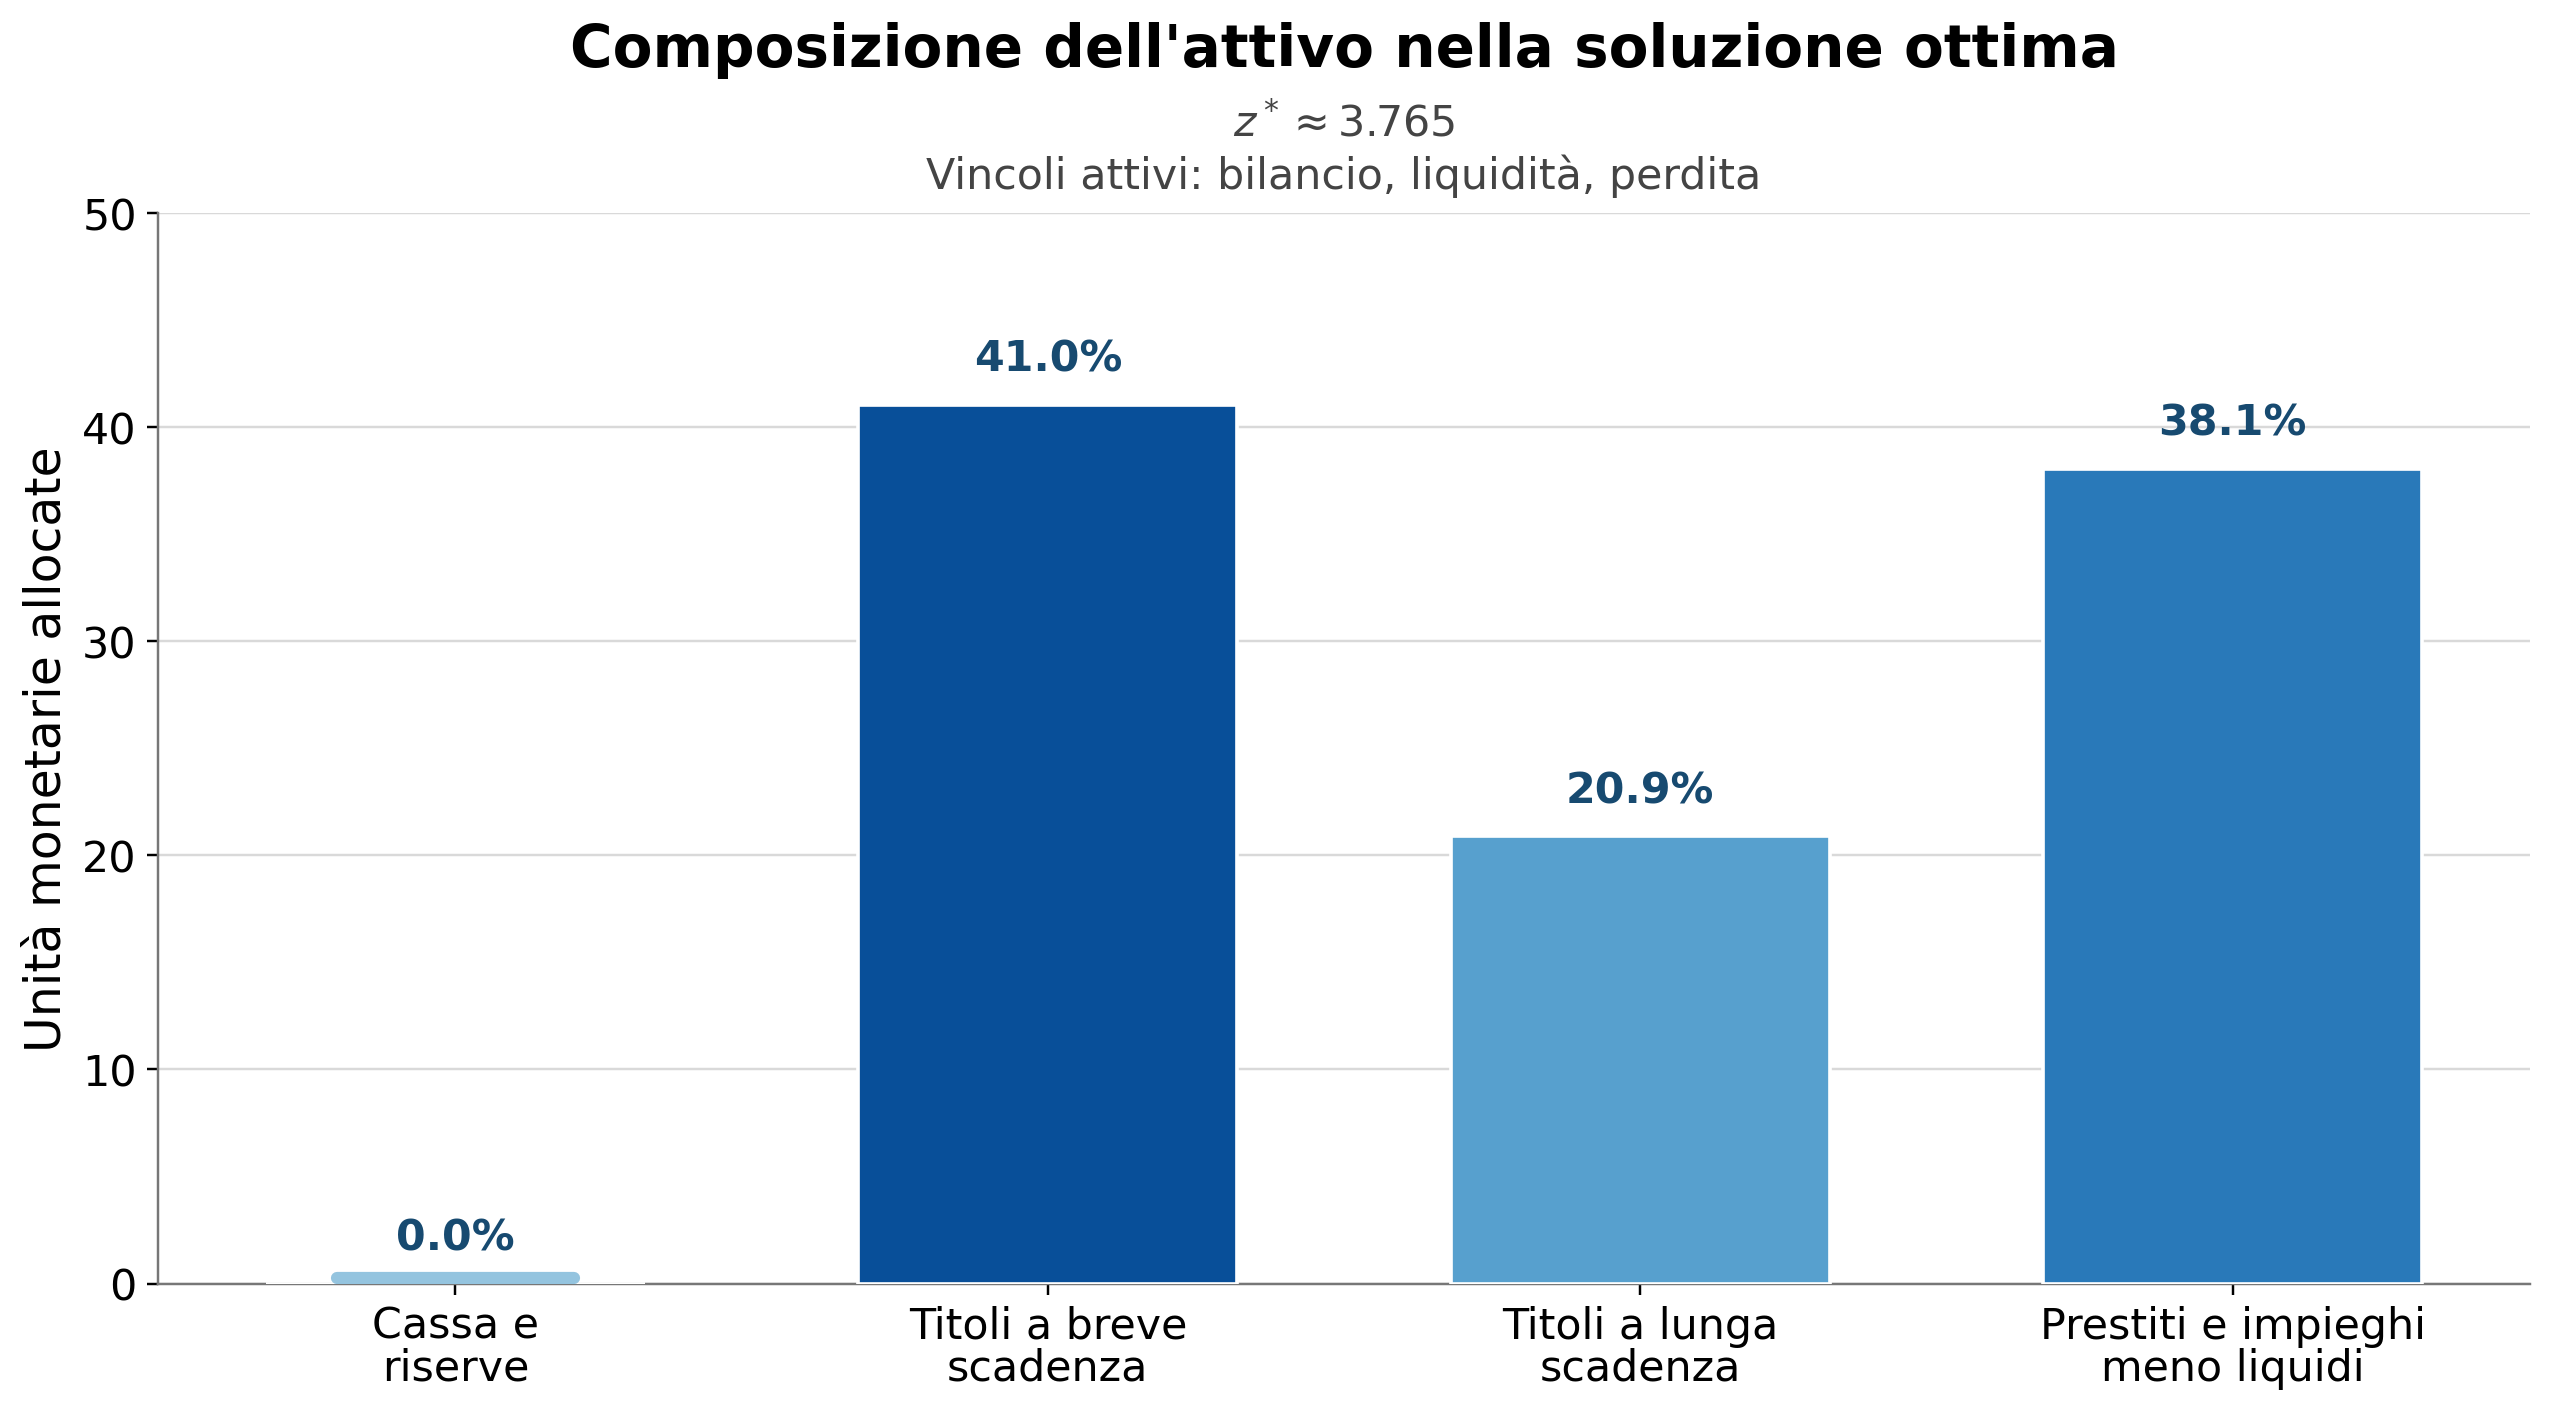
\includegraphics[width=0.72\textwidth]
{../graphics/Cap11_soluzione_ottima_allocazione.png}
\end{center}

\begin{stepitemize}
\item Il valore $z^{*}$ va letto nell'unit\`{a} dei coefficienti $c_j$: rendimento percentuale.
\end{stepitemize}

%TCIMACRO{\TeXButton{Transition: Box Out}{\transboxout}}%
%BeginExpansion
\transboxout%
%EndExpansion
%TCIMACRO{\TeXButton{EndFrame}{\end{frame}}}%
%BeginExpansion
\end{frame}%
%EndExpansion

%*****************************

\subsection{Che cosa rivelano i vincoli attivi}%

%TCIMACRO{\TeXButton{BeginFrame}{\begin{frame}}}%
%BeginExpansion
\begin{frame}%
%EndExpansion

\QTR{frametitle}{Che cosa determina davvero la composizione}

%TCIMACRO{\TeXButton{Transparency}{\setbeamercovered{transparent=20}}}%
%BeginExpansion
\setbeamercovered{transparent=20}%
%EndExpansion

\begin{center}
{\small
\begin{tabular}
[c]{lccc}\hline
\textbf{Requisito} & \textbf{Valore} & \textbf{Limite} & \textbf{Margine}%
\\\hline
Bilancio & $100$ & $=100$ & $0$ \quad attivo\\
Liquidit\`{a} & $55.00$ & $\geq55$ & $0$ \quad attivo\\
Perdita sotto stress & $7.00$ & $\leq7$ & $0$ \quad attivo\\
Titoli a lunga scadenza & $20.896$ & $\leq30$ & $9.104$\\\hline
\end{tabular}
}
\end{center}

\medskip

\begin{stepitemize}
\item La decisione non \`{e} arrestata dal limite di concentrazione, ma
dalla combinazione tra \textbf{fabbisogno di liquidit\`{a}} e
\textbf{capacit\`{a} di assorbire perdite}. Questa informazione \`{e}
economicamente pi\`{u} significativa del solo valore di $z^{*}$.

\item Cassa nulla non significa cassa inutile: con questi coefficienti il
requisito di liquidit\`{a} pu\`{o} essere soddisfatto attraverso i titoli a
breve, che rendono di pi\`{u}. Se la banca ritiene necessaria una dotazione
minima, deve scriverla come vincolo: $x_1\geq C_{\min}$.
\end{stepitemize}

\medskip

\begin{center}
{\small La soluzione ottima mette in evidenza non soltanto la decisione
preferita dal modello, ma anche i requisiti economici che il modello non
contiene ancora.}
\end{center}

%TCIMACRO{\TeXButton{Transition: Box Out}{\transboxout}}%
%BeginExpansion
\transboxout%
%EndExpansion
%TCIMACRO{\TeXButton{EndFrame}{\end{frame}}}%
%BeginExpansion
\end{frame}%
%EndExpansion

%*****************************

\section{Il costo di una maggiore prudenza}

%*****************************

\subsection{La funzione del valore ottimo}%

%TCIMACRO{\TeXButton{BeginFrame}{\begin{frame}}}%
%BeginExpansion
\begin{frame}%
%EndExpansion

\QTR{frametitle}{Che cosa accade se il requisito diventa pi\`{u} severo}

%TCIMACRO{\TeXButton{Transparency}{\setbeamercovered{transparent=20}}}%
%BeginExpansion
\setbeamercovered{transparent=20}%
%EndExpansion

Il livello $Q_{\min}=55$ non \`{e} prodotto dal modello: \`{e} un dato
deciso prima della soluzione. Trattiamolo come un \textbf{parametro} $Q$ e
indichiamo con $z^{*}(Q)$ il migliore risultato compatibile con esso.

\medskip

Se $Q_2>Q_1$, ogni decisione che soddisfa il requisito pi\`{u} severo
soddisfa anche quello pi\`{u} blando:
\[
\mathcal{X}(Q_2)\subseteq\mathcal{X}(Q_1)
\qquad\Longrightarrow\qquad
z^{*}(Q_2)\leq z^{*}(Q_1).
\]

\medskip

\begin{stepitemize}
\item Il risultato non afferma che una maggiore liquidit\`{a} sia
indesiderabile. Afferma che un requisito pi\`{u} severo pu\`{o} escludere
alcune allocazioni redditizie.

\item La riduzione di $z^{*}(Q)$ misura il \textbf{costo opportunit\`{a}}
della maggiore prudenza \emph{all'interno del modello}.
\end{stepitemize}

%TCIMACRO{\TeXButton{Transition: Box Out}{\transboxout}}%
%BeginExpansion
\transboxout%
%EndExpansion
%TCIMACRO{\TeXButton{EndFrame}{\end{frame}}}%
%BeginExpansion
\end{frame}%
%EndExpansion

%*****************************

\subsection{Analisi numerica e costo marginale}%

%TCIMACRO{\TeXButton{BeginFrame}{\begin{frame}}}%
%BeginExpansion
\begin{frame}%
%EndExpansion

\QTR{frametitle}{Il costo marginale della liquidit\`{a}}

%TCIMACRO{\TeXButton{Transparency}{\setbeamercovered{transparent=20}}}%
%BeginExpansion
\setbeamercovered{transparent=20}%
%EndExpansion

\begin{center}
{\small
\begin{tabular}
[c]{ccl}\hline
$Q$ & $z^{*}(Q)$ & \textbf{Composizione ottima}\\\hline
$55$ & $3.7649$ & $(0;\;41.045;\;20.896;\;38.060)$\\
$60$ & $3.5896$ & $(0;\;46.269;\;25.373;\;28.358)$\\
% $65$ & $3.4142$ & $(0;\;51.493;\;29.851;\;18.657)$\\
$70$ & $3.2357$ & $(0;\;58.571;\;30.000;\;11.429)$\\
$80$ & $2.8750$ & $(0;\;75.000;\;25.000;\;0)$\\\hline
\end{tabular}
}
\end{center}

\begin{center}
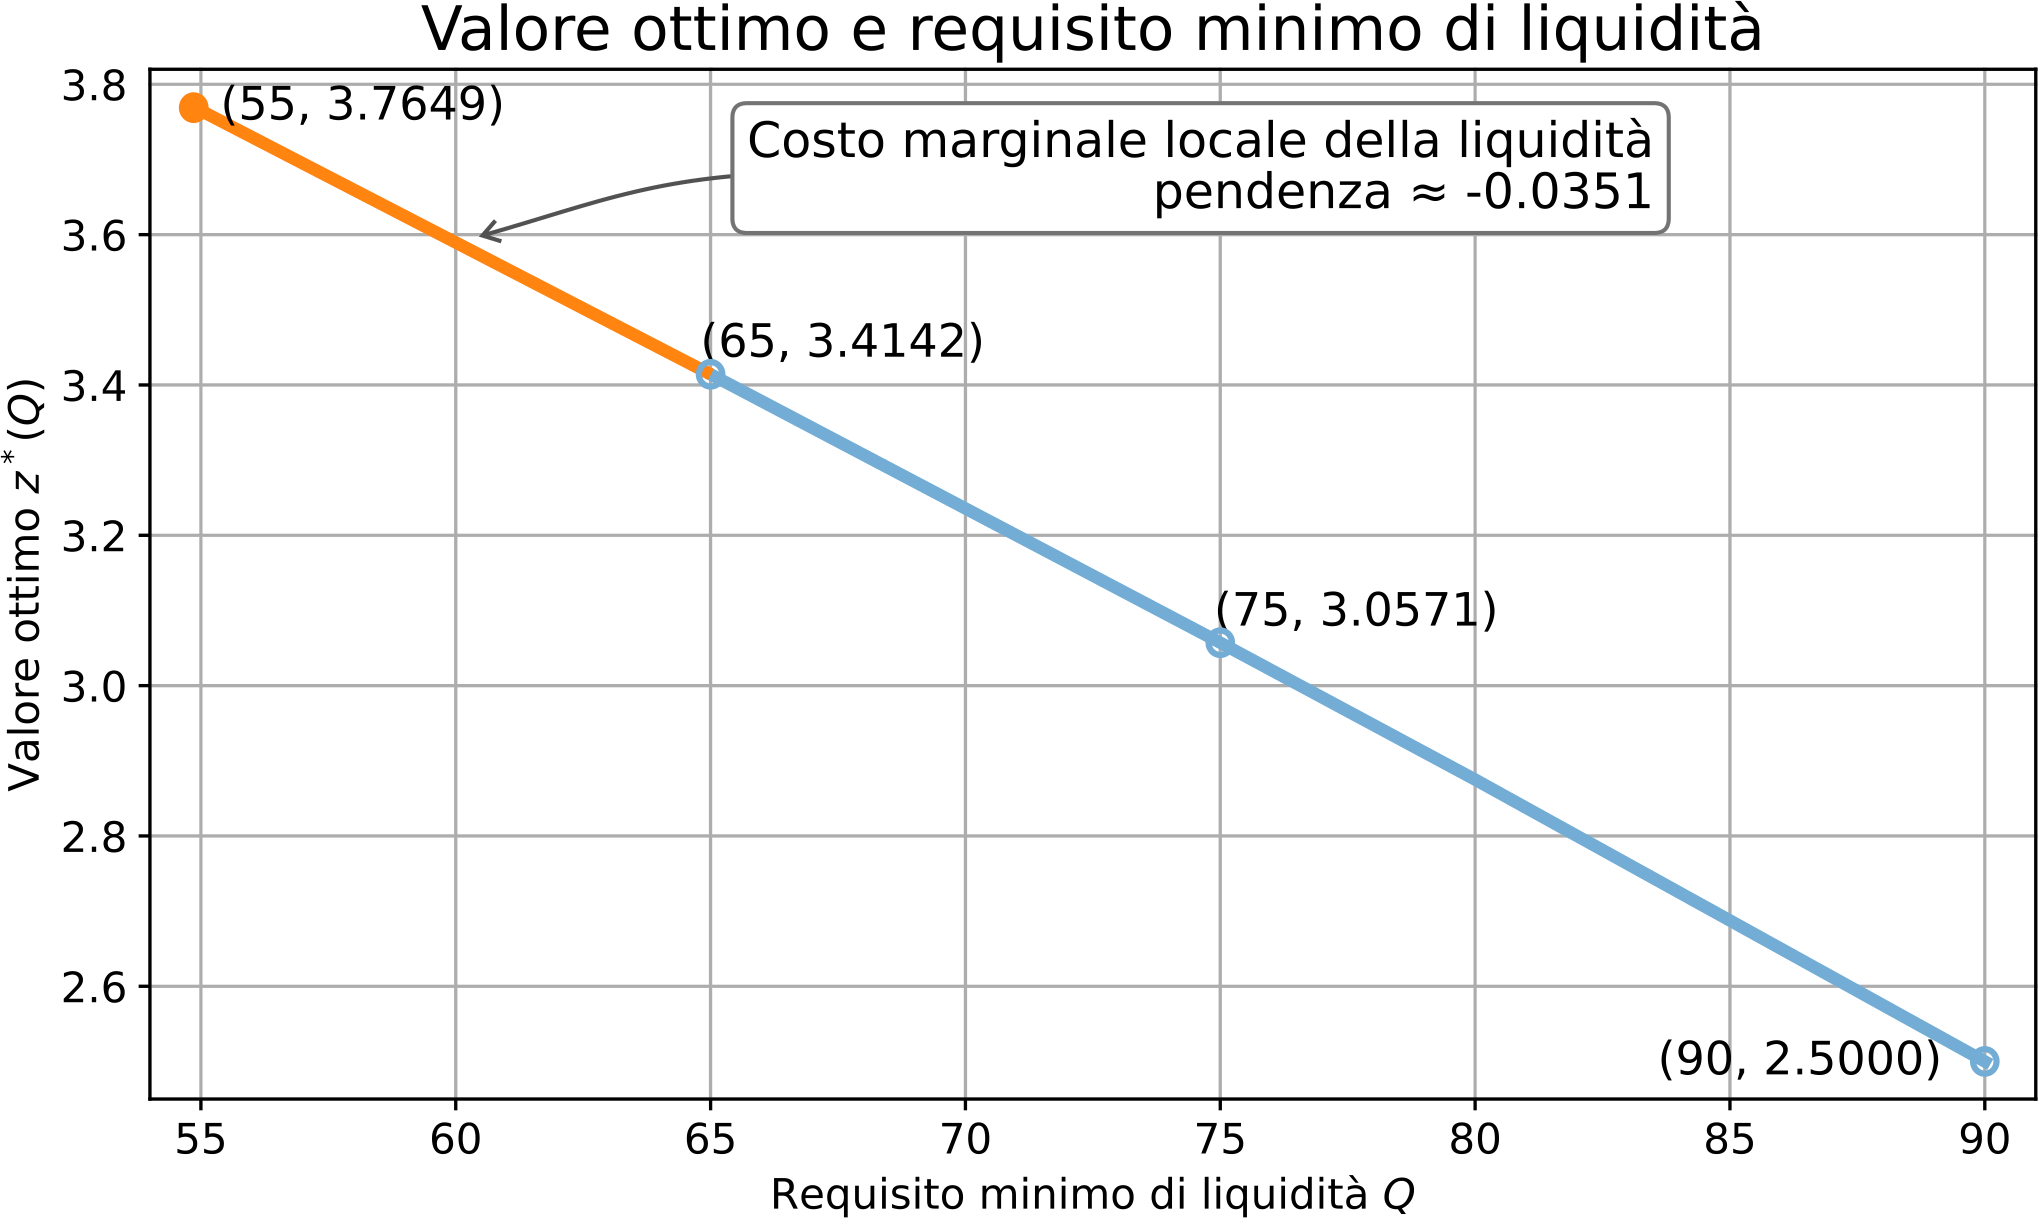
\includegraphics[width=0.58\textwidth]
{../graphics/Cap11_valore_ottimo_liquidita.png}
\end{center}

\smallskip

Tra $Q=55$ e $Q=56$ il valore ottimo scende da $3.7649$ a $3.7299$: una
unit\`{a} aggiuntiva di liquidit\`{a} costa circa $0.0351$.

%TCIMACRO{\TeXButton{Transition: Box Out}{\transboxout}}%
%BeginExpansion
\transboxout%
%EndExpansion
%TCIMACRO{\TeXButton{EndFrame}{\end{frame}}}%
%BeginExpansion
\end{frame}%
%EndExpansion

%*****************************

\subsection{Una valutazione locale}%

%TCIMACRO{\TeXButton{BeginFrame}{\begin{frame}}}%
%BeginExpansion
\begin{frame}%
%EndExpansion

\QTR{frametitle}{Come leggere il costo marginale}

%TCIMACRO{\TeXButton{Transparency}{\setbeamercovered{transparent=20}}}%
%BeginExpansion
\setbeamercovered{transparent=20}%
%EndExpansion

\begin{stepitemize}
\item \textbf{Non \`{e} una spesa}. Nessun esborso contabile: \`{e} il
rendimento massimo al quale il modello deve rinunciare per rispettare un
requisito leggermente pi\`{u} severo.

\item \textbf{La composizione si ricompone}. Le risorse migrano verso i
titoli a breve, che hanno liquidabilit\`{a} elevata; si riducono gli
impieghi meno liquidi, che passano da $38$ a zero.

\item \textbf{Il valore \`{e} locale}. Vale finch\'{e} non cambia
l'insieme dei vincoli che determinano la soluzione. A $Q=70$ i titoli a
lunga raggiungono il limite di concentrazione: da quel punto in poi il
costo di un'ulteriore unit\`{a} \`{e} maggiore e va ricalcolato.
\end{stepitemize}

\medskip

\begin{center}
{\small L'analisi marginale risponde alla domanda: quanto risultato viene
sacrificato imponendo una piccola variazione del requisito? Non risponde
alla domanda normativa su quale debba essere il livello corretto di
liquidit\`{a}, che richiede valutazioni sul rischio dei deflussi e sulla
stabilit\`{a} della raccolta.}
\end{center}

%TCIMACRO{\TeXButton{Transition: Box Out}{\transboxout}}%
%BeginExpansion
\transboxout%
%EndExpansion
%TCIMACRO{\TeXButton{EndFrame}{\end{frame}}}%
%BeginExpansion
\end{frame}%
%EndExpansion

%*****************************


%*****************************
\end{document}